
\section{Discussion}
\label{sec:discussion}

In this section, we discuss the physical implications of our empirical
findings regarding bow shock shapes.  Our most reliable result is the
average shape of the OB bow shocks from the 227 MIPSGAL sources with
quality rating of 3~stars or higher.  This yields mean values of
\(\Pi = 1.78 \pm 0.06\) and \(\Lambda = 1.72 \pm 0.02\), or median values of
\(\Pi = 1.57\) and \(\Lambda = 1.69\).  The uncertainty quoted on the mean
values is the ``standard error of the mean'':
\(\text{sem} = \sigma / \sqrt{n}\), where \(\sigma\) is the rms dispersion and
\(n\) is the number of sources.  Note that in the case of the
planitude \(\text{sem}(\Pi) = 0.06\) is considerably smaller than
\(\text{mean}(\Pi) - \text{median}(\Pi) = 0.21\), so the latter would be a
more conservative estimate of the uncertainty.\footnote{This is
  because the distribution of \(\Pi\) is approximately log-normal, which
  yields a significant tail towards high values when converted to
  linear space.}  These values can be compared with the predictions of
the thin-shell wilkinoid model \citep{Wilkin:1996a}, which are
\(\Pi = 1.67\), \(\Lambda = 1.73\) when the bow shock axis lies in the plane
of the sky (following Paper~0, this is defined as the zero point of
the inclination angle, \(i\)).  When the axis is inclined, both
planitude and alatude are predicted to decrease but not by very much,
tending to \(\Pi = 1.5\), \(\Lambda = 1.63\) as
\(\abs{i} \to \ang{90}\) (see \S~5.3 of Paper~0).  The median observed
value\footnote{In the presence of outliers, the median is a more
  robust estimate of the central tendency than is the mean.} falls
squarely inside this range for both the planitude and alatude, which
is a remarkable triumph for the \citet{Wilkin:1996a} model.

On the other hand, turning now to the \emph{variety} of bow shock
shapes, we see that the wilkinoid can no longer explain our results.
The rms dispersions of the planitude and alatude distributions for the
MIPSGAL sources are \(\sigma(\Pi) = 0.87\) and
\(\sigma(\Lambda) = 0.30\) (Tab.~\ref{tab:big-p}), which are respectively 5 times
and 3 times larger than the total range of variation of \(\Pi\) and
\(\Lambda\) predicted for the wilkinoid surface.  Although some of the
dispersion is due to uncertainties in the observations and the fitting
algorithm, this contribution is expected to be small, especially for
the larger, well-resolved sources, for which systematic uncertainties
in the methods for determining \(\Pi\) and \(\Lambda\) will
dominate. Conservative upper limits to the relative size of these
uncertainties were estimated in \S~7 of Paper~0 to be \(< 20\%\) for
\(\Pi\) and \(< 10\%\) for \(\Lambda\), whereas the observed dispersions are
roughly twice as large: \(\sigma(\Pi)/\Pi = 55\%\) and
\(\sigma(\Lambda)/\Lambda = 18\%\).  Furthermore, the variations in planitude and
alatude are readily apparent by eye, as is demonstrated by the example
bow shock images shown in Figure~\ref{fig:mipsgal-shapes}b.  Sources
such as K123 have very typical shapes and fall near the center of the
\(\Pi\)--\(\Lambda\) distribution, whereas high-\(\Pi\) sources such as K447 have
a very flat apex region, while low-\(\Pi\) sources such as K566 have a
pointier, almost triangular apex.  High-\(\Lambda\) sources, such as K517,
have very open wings that bend away from the star, while
low-\(\Lambda\) sources such as K489 have closed wings and a semi-circular
appearance.


In Paper~0 we found that certain bow shock shapes can show a much
greater variation in their projected appearance as a function of
inclination angle than is seen for the wilkinoid.  For example, the
cantoids and ancantoids, which have asymptotically hyperbolic far
wings, can shift towards higher apparent planitude and alatude as the
inclination increases, generally with \(\Lambda \ge \Pi\) (Fig.~20 of Paper~0).
This might plausibly explain the vertical spur towards higher
\(\Lambda\) seen in the empirical distribution (\S~\ref{sec:ob-shapes}). A
different behavior is shown by bow shocks with very flat apex regions,
such as the MHD simulation from \citet{Meyer:2017a} that is analyzed
in the \S~6 of Paper~0.  This shows a high planitude \(\Pi\) when the
orientation is exactly edge-on, but \(\Pi\) decreases sharply along a
roughly horizontal track as the inclination \(\abs{i}\) increases
(Fig.~25 of Paper~0).  This is similar to the principal axis of
variation of the observed shapes (e.g.,
Fig.~\ref{fig:mipsgal-shapes}a).

If such variations in orientation do make a significant contribution
to the observed distribution of bow shock shapes in the
\(\Pi\)-\(\Lambda\) plane, then various predictions follow, which might be
observationally tested.  High-planitude sources with \(\Pi > 3\) would
be expected to have low inclinations, \(\abs{i} < \ang{30}\), whereas
high-alatude sources with \(\Lambda > 2\) would be expected to have high
inclinations, \(\abs{i} > \ang{45}\).  Unfortunately, determination of
the inclination for individual sources requires high resolution
spectroscopy of emission lines in order to map the kinematics of the
flow in the bow shock shell \citep[e.g.,][]{Henney:2013a}.  This is
not currently available for the majority of the MIPSGAL sources, which
are detected only by their dust continuum emission.  A further
prediction for the high-alatude sources is that the environmental flow
should be divergent rather than plane-parallel, in order to give a
cantoid shape instead of a wilkinoid.  This would tend to favor
``weather-vane'' cases, where the interstellar medium is flowing past
the star, and disfavor ``runaway'' cases, where the star is moving
through a static medium.  However, in \S~\ref{sec:corr-shape} we found
no significant difference in the shape distributions as a function of
the bow shock environment.  Figure~\ref{fig:mipsgal-uncorrelated}a
shows that the alatudes of sources that are facing \hii{} regions or
\SI{8}{\um} bright-rimmed clouds (and therefore might be expected to
be immersed in a champagne flow) are no higher than sources that are
isolated.


\begin{figure}
  (a)\\
  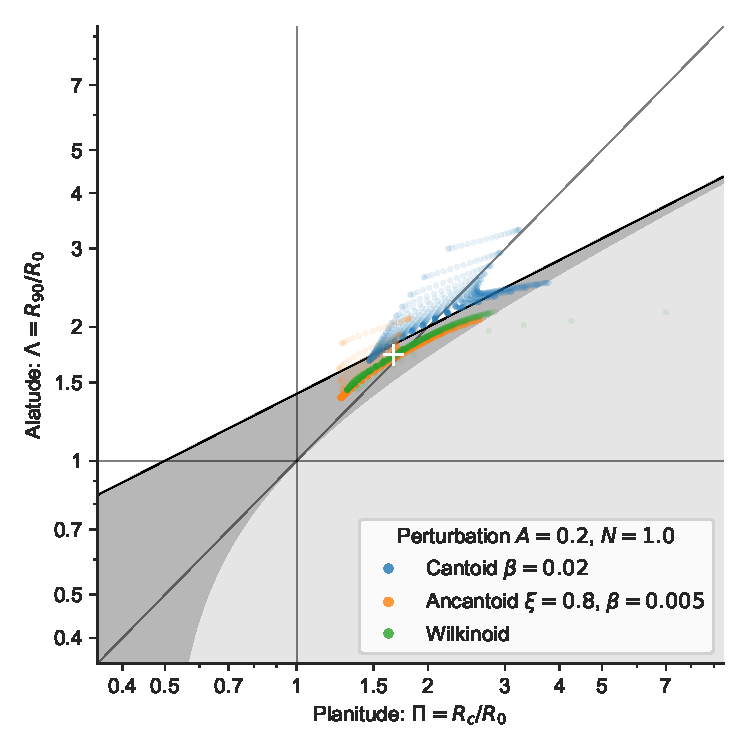
\includegraphics[width=\linewidth]
  {figs/wave-R90-vs-Rc-A020-N10}
  (b)\\
  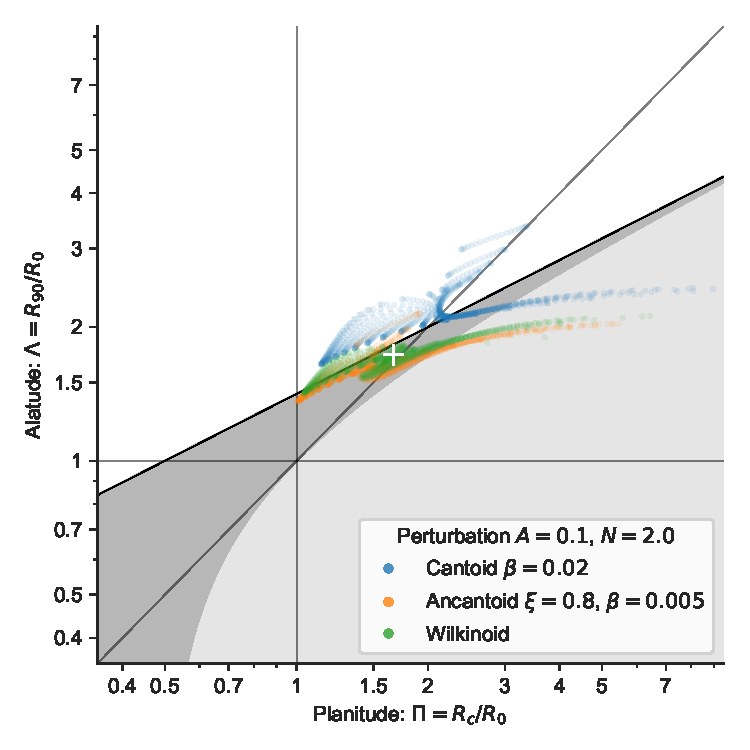
\includegraphics[width=\linewidth]
  {figs/wave-R90-vs-Rc-A010-N20}
  \vspace*{-\baselineskip}
  \caption{Diagnostic diagram for perturbed shapes from standing wave
    oscillations.  Each model is characterized by a base shape
    (colored symbols, as described in key) and an amplitude, \(A\),
    and wavenumber, \(N\), of the oscillation: (a)~breathing mode with
    \(N = 1\), \(A = 0.2\); (b)~curling mode with \(N = 2\),
    \(A = 0.1\) (see Fig.~\ref{fig:perturb-shapes} for the
    phase-dependent intrinsic shapes).  The plotted points show the
    varying planitude and alatude of the projected bow shock shapes
    with uniform sampling over an entire period of the oscillation and
    for varying inclinations (sampled according to an isotropic
    distribution of orientations).  Each individual point is plotted
    with a low opacity so that the crowding of points in certain
    regions of the plane can be appreciated.}
  \label{fig:perturb-Rc-R90}
\end{figure}

An alternative explanation for the variety of observed bow shock
shapes is that they are due to time-dependent perturbations to an
underlying base shape.  For instance, multiple studies have shown that
stellar bow shock shells can be unstable \citep{Dgani:1996a,
  Dgani:1996b, Blondin:1998a, Comeron:1998a, Meyer:2014a}, leading to
large amplitude oscillations in the shell shape.  The oscillations are
found to be most vigorous when the post shock cooling is highly
efficient, allowing the formation of a thin shell (see Paper~I).  Even
in cases where the shell is stable, oscillations may be driven by
periodic variations in the stellar wind mass-loss rate or velocity, or
by inhomogeneities in the ambient stream.  Rather than using a
particular dynamical model of these oscillations, we instead crudely
simulate their effect by assuming a constant amplitude standing wave
perturbation to the base shape, as described in
Appendix~\ref{sec:perturbed-bows}.  Example results are shown in
Figure~\ref{fig:perturb-Rc-R90} for an ensemble of bow shocks with
different orientations and phases of oscillation, considering three
different underlying base shapes.  It can be seen that modest
amplitudes of 10 to 20\% can give rise to a distribution in \(\Pi\) and
\(\Lambda\) similar to that observed for the MIPSGAL sources when the
oscillation wavelength is of the same order as the bow shock size.

An attractive feature of the oscillation hypothesis is that it
naturally explains why we find little correlation between the bow
shock shape and other source parameters (\S~\ref{sec:corr-shape}),
since the instantaneous shape at any instant is largely a matter of
chance rather than being due to any intrinsic property of the source.
The one significant correlation that we do find is that the alatude
distribution is broader for bow shocks with larger angular sizes.
This might be explained if the relative amplitude of oscillations were
higher for sources with more powerful winds. \citet{Meyer:2016a} in
their Fig.~2 plot the ``axis ratio'' (which is our \(\Lambda^{-1}\)) as a
function of apex distance for a large set of hydrodynamic bow shock
simulations.  They find the most unstable bow shocks (with the largest
spread in \(\Lambda\)) to be those associated with the highest mass stars in
a relatively dense medium, which have apex distances of
\SIrange{0.3}{1}{pc}.  This corresponds to \(R_0 > 15''\) for
distances less than \SI{4}{kpc}, which is larger than the median
angular size for the MIPSGAL sources, making this a plausible explanation for our statistical result.
% However, in that case it
% is hard to understand why no such variation is seen in the width of
% the planitude distribution.

We now address the difference in shape distribution between the
different classes of source.  Compared with the OB star bow shocks,
the cool star sample from \citet{Cox:2012a}\footnote{Three of these
  sources are high-mass red supergiant (RSG) stars, while the
  remaining 13 are intermediate-mass asymptotic giant branch (AGB)
  stars.} shows a significantly smaller alatude of
\(\Lambda = 1.41 \pm 0.03\) (see
Fig.~\ref{fig:herschel-compare-mipsgal}).\footnote{Although the
  planitude also appears to be slightly smaller, this is not very
  statistically significant due to the small number of cool star
  sources and the large width of the OB star planitude distribution.}
Such a closed shape for the wings is inconsistent with the wilkinoid
value of \(\Lambda = \text{\numrange{1.63}{1.73}}\), which is surprising
given that the emission shells in these sources are relatively narrow
(Figs.~\ref{fig:herschel-arc-fits}
and~\ref{fig:herschel-arc-fits-poor}), so one might have thought that
the thin-shell approximation of \citet{Wilkin:1996a} would be
\emph{more} appropriate than for the OB stars, but this is clearly not
the case.  One possible explanation for this might be that the bow
shocks have not had time to reach a steady-state configuration, as was
suggested by \citet{Mohamed:2012a} for the case of \(\alpha\)~Ori.  The
dynamical timescales, \(R_0 / V\wind\), for the cool star bow shocks
are of order \SI{e4}{yr} and numerical simulations \citetext{e.g.,
  Fig.~11 of \citealp{Mohamed:2012a} and Fig.~2 of
  \citealp{van-Marle:2014a}} show that the bow shock wings take of
order \SIrange{3e4}{e5}{yr} to fully unfold.  However, this is still
short compared with typical RSG and AGB lifetimes, so while it might
apply to a single source it does not work as an explanation for an
entire class of sources, especially given that the alatude and
planitude distributions for these sources are so narrow
(Fig.~\ref{fig:herschel-compare-mipsgal}).  A more promising
explanation is that the shape difference reflects a different origin
for the infrared-emitting dust.  In hot stars, the stellar wind is
dust-free, so the only dust shell comes from the interstellar medium
and lies outside the astropause (contact discontinuity).  In cool
stars, the stellar wind is also dusty, which could give rise to
significant infrared emission from near the stellar wind's termination
shock, as has been found from hydrodynamic simulations
\citep{Meyer:2014b}.  This is certainly the case for at least one of
our cool star sources, the C-AGB star CW~Leo (IRC+10216), where
ultraviolet GALEX observations \citep{Sahai:2010a} clearly show
\emph{both} the outer shock and the wind termination shock, and
comparison with the Herschel images demonstrate that the infrared dust
emission is associated with the latter.


% However, in order for the dust emission arc to be less open than the
% wilkinoid case, one would require the shocked stellar wind shell to be
% relatively thick, which means that either the Mach number must be low
% or the post-shock cooling must be inefficient (see Paper~I).  In some
% red supergiants, the stellar wind is heated and photoionized by the
% ambient radiation field before reaching the bow shock
% \citep{Morris:1983a, Mackey:2014a}, which would tend to produce a low
% Mach number shock.

In the case of the Orion Nebula bow shocks
(\S~\ref{sec:stat-emiss-line}), we have the opposite situation, where
the alatude and planitude are both significantly larger on average
than for the OB star sources (Fig.~\ref{fig:ll-compare-mipsgal}).  On
the face of it, this is surprising because there are two differences
between the source classes that would tend to work in the other
direction.  First, many of the Orion sources are proplyds, or
externally illuminated photoevaporating disks \citep{ODell:2008b}, in
which the inner wind is not isotropic but instead is mildly
concentrated towards the symmetry axis \citep{Garcia-Arredondo:2001a},
so that simple models predict an \textit{ancantoid} shape
\citep[\S~5]{Tarango-Yong:2018a} that is less open than for an
isotropic wind.  Second, as was the case with the cool star sources,
both the shocked inner wind and the shocked outer stream are expected
to contribute to the emission arcs.  Indeed, in several of the sources
of Figure~\ref{fig:ll-arcs} (LL~3, 116--3101, 266-558, 308-3036, and
LL~5), a two-component emission structure is apparent.  In the case of
the cool star bow shocks, we invoked this as a possible explanation of
their \emph{low} alatude (see previous paragraph), so
some stronger countervailing factor is necessary in order to explain
why the opposite is seen in the Orion Nebula bow shocks.


Four possible origins for this countervailing factor suggest
themselves: (i)~the external flow may be more divergent in the Orion
sources; (ii)~the Mach number of the external flow may be
systematically lower; (iii)~the fact that the arcs are observed in
recombination line emission instead of dust continuum may cause
different observational biases; (iv)~the shapes may be influenced by
collimated jet outflows from the young stars.  We now address each of
these in turn.

In case~(i) one would expect \(\Pi\) and \(\Lambda\) to be positively
correlated with \(R_0/D\), where \(R_0\) is the bow shock size
(star--apex separation) and \(D\) is the distance from the center of
divergence of the external flow.  In \S~\ref{sec:stat-emiss-line} we
found that these are indeed correlated, but only weakly.  A more
serious objection to this idea is that according to hypersonic
thin-shell models \citep{Canto:1996} the momentum ratio parameter
\(\beta\) must be relatively large in order to give significantly open bow
shock shapes.  From Figure~20 of Paper~0 we see that
\(\beta > \num{e-3}\) is required in order to give
\(\Pi, \Lambda > 2\).  However, for small \(\beta\) one has
\(\beta \approx (R_0/D)^2\), which yields \(\beta = \num{4e-6}\) to \num{3e-4} for
our sources, so that divergence ought to have little effect on the
shapes.

Case~(ii) arises from the fact that, if the hypersonic assumption is
relaxed, then the opening angle between the outer bow shock and the
contact discontinuity in the wings becomes increasingly large as the
Mach number, \(\M\), drops towards unity.  This is a consequence of
the \textit{shock polar} relation for oblique shocks \citep[\S\S~92
and 113]{Landau:1987a} and applies to both the radiative and
non-radiative case.  It will tend to produce more open shapes, at
least in the case that the emission is dominated by the outer shell.
At the same time, the relative thickness of the shell, \(h/R_0\), is
predicted to increase as \(\M\) decreases \citetext{e.g., eq~[35] of
  Paper~I}.  We have therefore measured \(h/R_0\) for the Orion
sources, finding values ranging from \numrange{0.3}{0.8} with median
of \num{0.5}.  We have not measured \(h/R_0\) for the full MIPSGAL
sample, but Figure~11 of Paper~III gives the values for the sub-sample
of OB bow shocks studied by \citep{Kobulnicky:2018a}.  The median
value is 0.2, implying thinner shells than in the Orion Nebula bow
shocks, which lends support to the idea that the Mach number may be
lower in the latter.  However, among the Orion sources we find that
\(h/R_0\) is completely uncorrelated with either \(\Pi\) or
\(\Lambda\) (\(r = 0.02\) and \(-0.05\), respectively).

Case~(iii) attempts to explain the difference in shapes as a result of
an ``optical illusion'' whereby the OB star bow shocks are in reality
more open than they appear. The hydrogen recombination line surface
brightness from an isothermal shell is proportional to the emission
measure (line of sight integral of the product of proton and electron
densities), whereas the mid-infrared surface brightness is not simply
proportional to the dust column density, since it results from the
reprocessing of stellar radiation.  For typical bow shock grain
temperatures \citetext{\(T = 50\) to \SI{100}{K},
  \citealp{Kobulnicky:2017a}} the \SI{24}{\um} band used for the OB
star sample lies on the short wavelength Wien side of the dust
emission spectrum, which gives a very steep radial dependence of the
emissivity.  \citet{Acreman:2016a} calculate synthetic emission maps
from hydrodynamical simulations and show that, even for a relatively
thin bow shock shell, the emission arc seen in H\(\alpha\) tends to be more
open than the arc seen in the mid-infrared (see their Fig.~3).  The
effect should be even larger for thicker shells, as demonstrated by
\citet{Mackey:2016a}, who simulate the subsonic motion of an O star
through its \hii{} region and show that this can give rise to an
\emph{apparent} bow shock at \SI{24}{\um} even when there is no
corresponding dense shell at all.

Finally, case~(iv) arises from the observation that several of the
Orion sources possess high velocity (\(> \SI{100}{km.s^{-1}}\))
collimated jets \citep{Bally:2006a}, which produce strings of emission
knots that partially overlap the wings of the bow shock.  In the case
of 109--246, LL~1, LL~4, LL~5, and LL~6, the projected jet axis is
roughly perpendicular to the projected bow shock axis, and two of
these (109--246 and LL~6) have the most extreme high values of \(\Pi\)
and \(\Lambda\).  There are several other Orion Nebula bow shock sources
with perpendicular jets (LL~2, 203--3039, 261--3018, 344--3020, and
LL~7), which we omitted from our sample because of difficulty in
measuring \(\Lambda\), but the majority also have large planitudes
\(\Pi > 5\). Only one source, 4468--605, has a jet oriented parallel to
the bow shock axis, and this has the smallest \(\Pi\) and third-smallest
\(\Lambda\) of the sample.  The circumstantial evidence thus points towards
the jets playing some role in shaping the bow shocks when they are
oriented perpendicular to the axis, even though we took care when
tracing the bow shock ridges to avoid any region with superimposed jet
knots.  This would break the cylindrical symmetry of the bow shock,
which should have a kinematic signature.  However, in the only two
sources that have been studied kinematically \citep{Henney:2013a}, the
bow shock shell does not show any sign of the red/blue asymmetry that
is seen in the jet knots, which argues against any such association.

%%% Local Variables:
%%% mode: latex
%%% TeX-master: "obs-bowshocks"
%%% End:
